\begin{center}
\footnotesize\noindent\fbox{
	\parbox{\textwidth}{
	Utilizzare le function degli Esercizi 4.1 e 4.6 per graficare l'approssimazione della funzione di Runge sull'intervallo \([-6, 6]\), per \(n = 2, 4, 6, \ldots, 40\). \\ \\Stimare numericamente l'errore commesso in funzione del grado \textit{n} del polinomio interpolante.
	}
}\end{center}

\noindent Di seguito i grafici che mostrano i polinomi interpolanti di
grado \textit{n} calcolati usando come punti di interpolazione quelli
corrispondenti alle \textit{n} ascisse di Chebyshev.

% brutto brutto brutto

\begin{center}
	\(n=2\) \\
	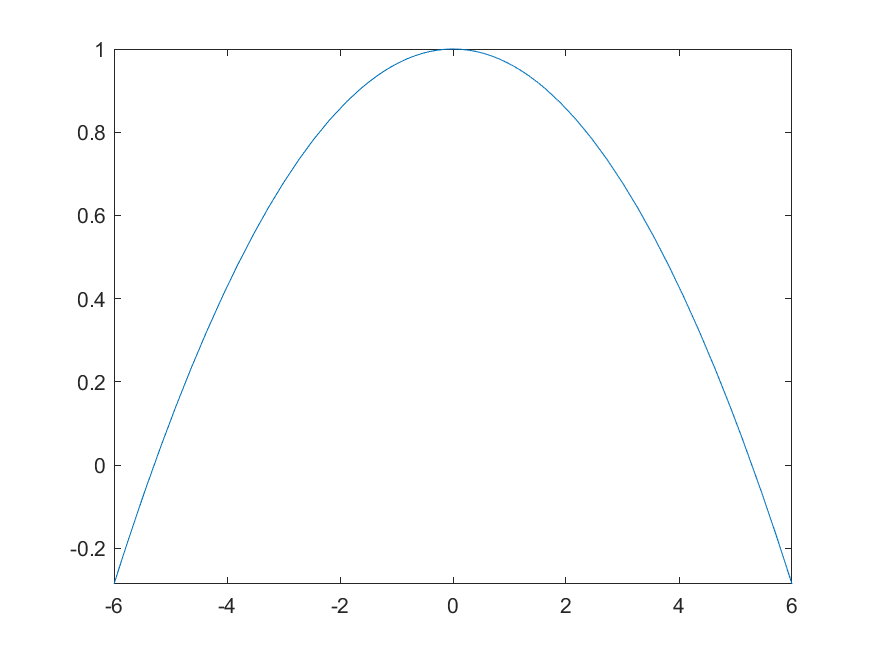
\includegraphics[scale=0.55]{cap4/4_7/2.png}
\end{center}

\begin{center}
	\(n=4\) \\
	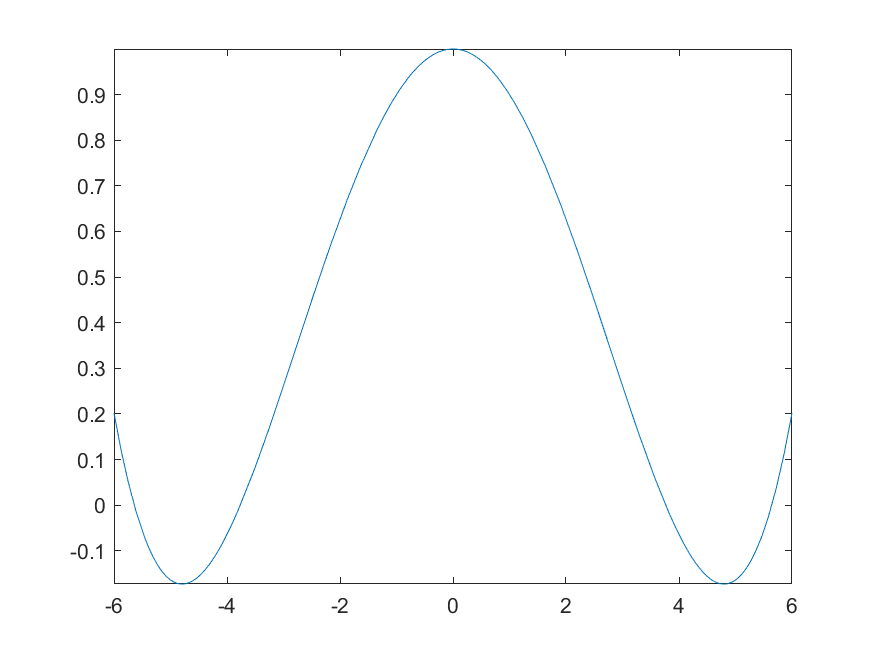
\includegraphics[scale=0.55]{cap4/4_7/4.png}
\end{center}

\vspace{0.2cm}

\begin{center}
	\(n=6\) \\
	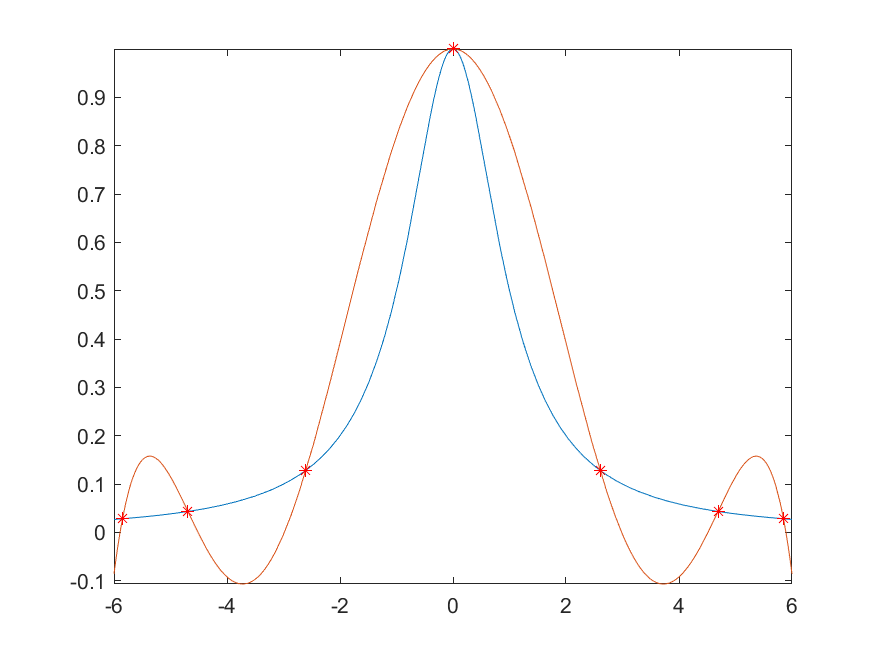
\includegraphics[scale=0.55]{cap4/4_7/6.png}
\end{center}

\begin{center}
	\(n=8\) \\
	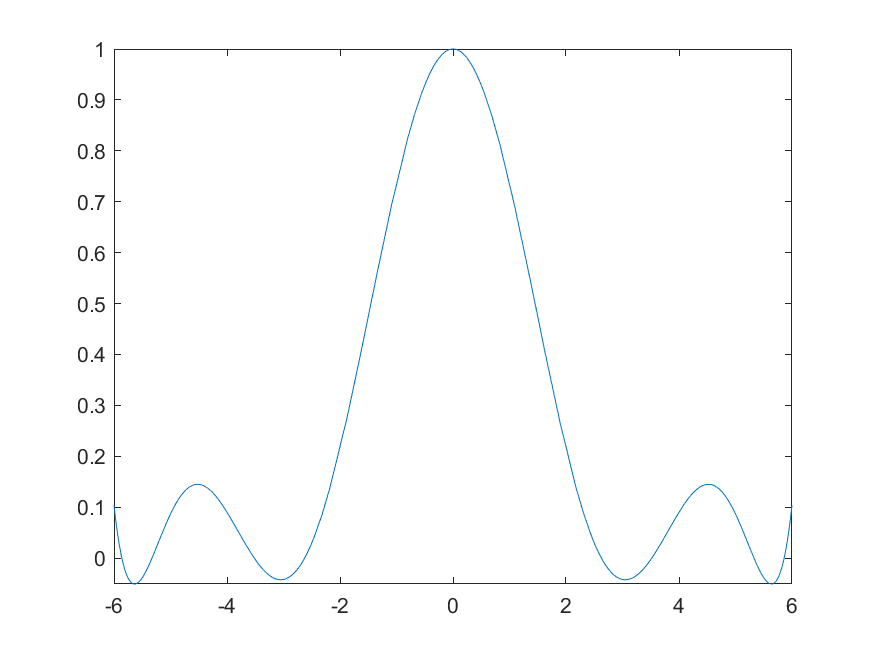
\includegraphics[scale=0.55]{cap4/4_7/8.png}
\end{center}

\begin{center}
	\(n=10\) \\
	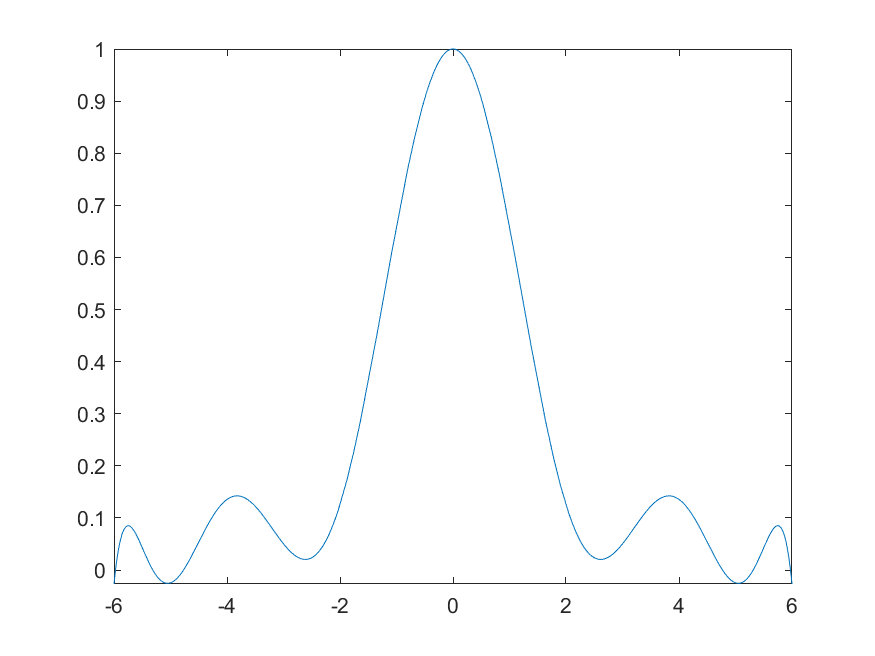
\includegraphics[scale=0.55]{cap4/4_7/10.png}
\end{center}

\begin{center}
	\(n=12\) \\
	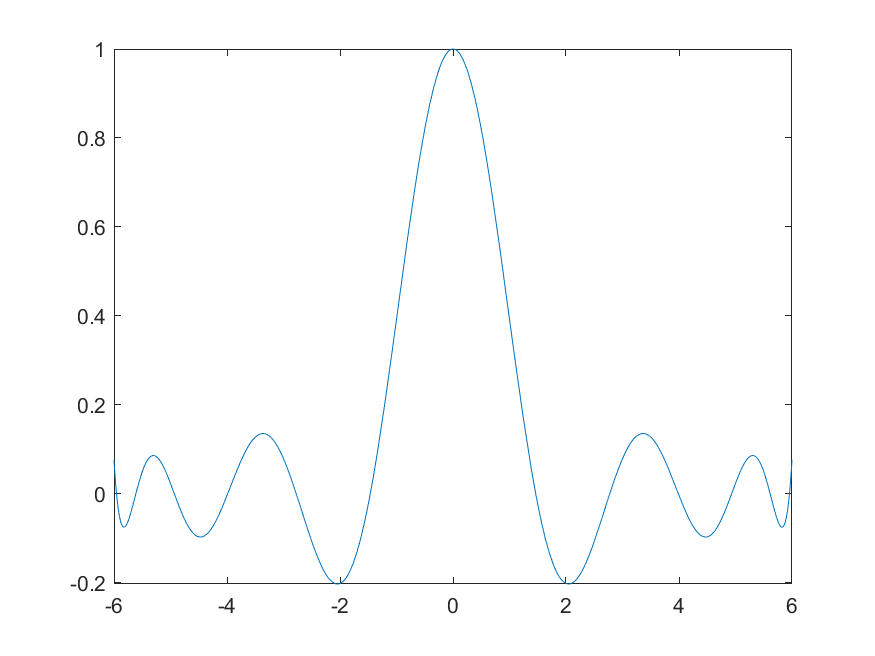
\includegraphics[scale=0.55]{cap4/4_7/12.png}
\end{center}

\begin{center}
	\(n=14\) \\
	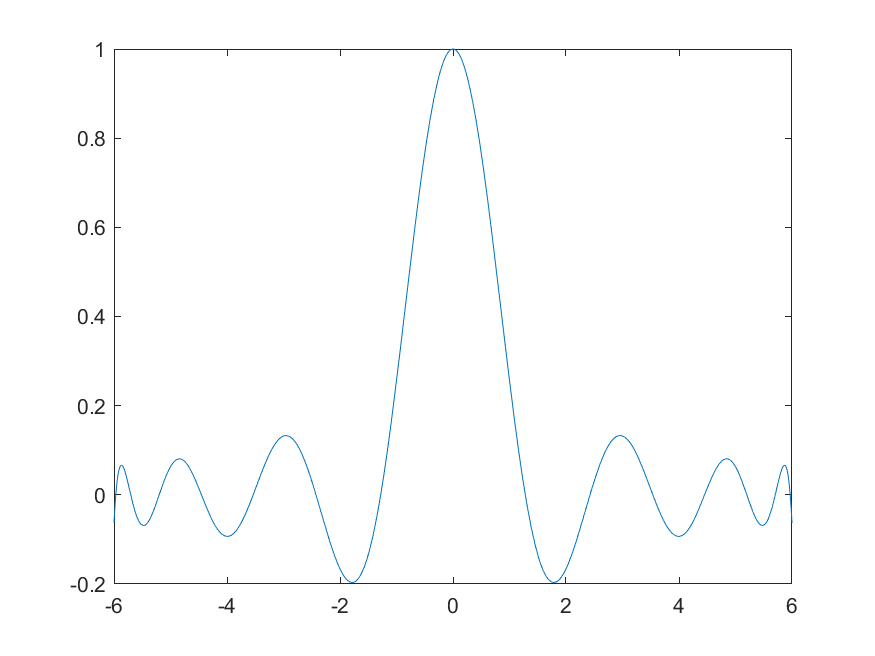
\includegraphics[scale=0.55]{cap4/4_7/14.png}
\end{center}

\begin{center}
	\(n=16\) \\
	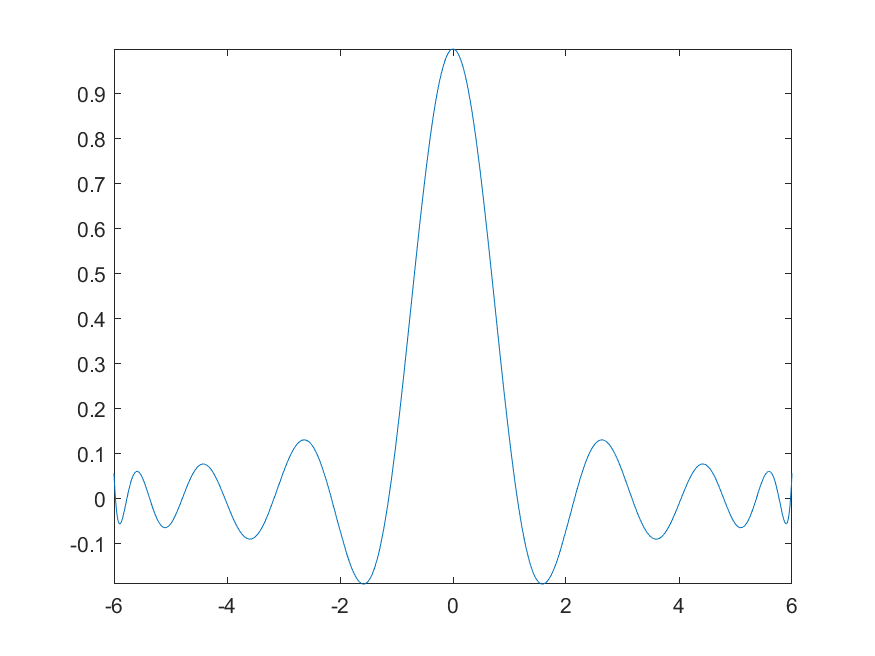
\includegraphics[scale=0.55]{cap4/4_7/16.png}
\end{center}

\begin{center}
	\(n=18\) \\
	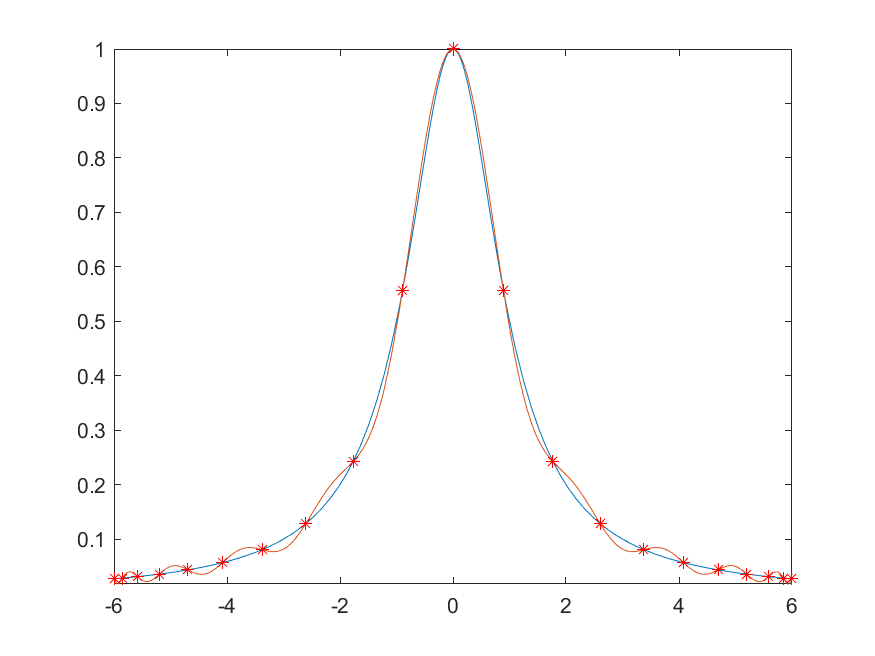
\includegraphics[scale=0.55]{cap4/4_7/20.png}
\end{center}

\begin{center}
	\(n=20\) \\
	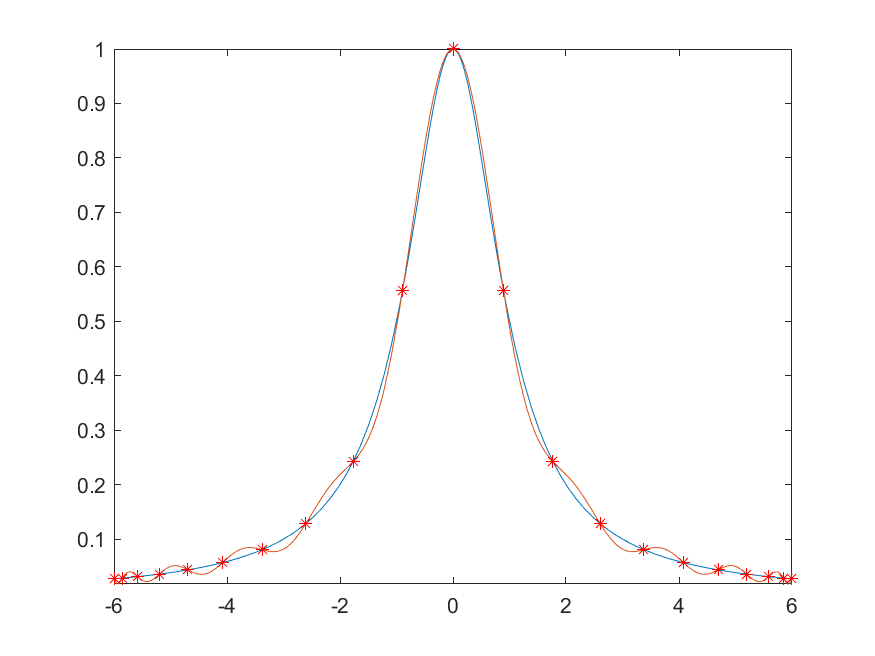
\includegraphics[scale=0.55]{cap4/4_7/20.png}
\end{center}

\begin{center}
	\(n=40\) \\
	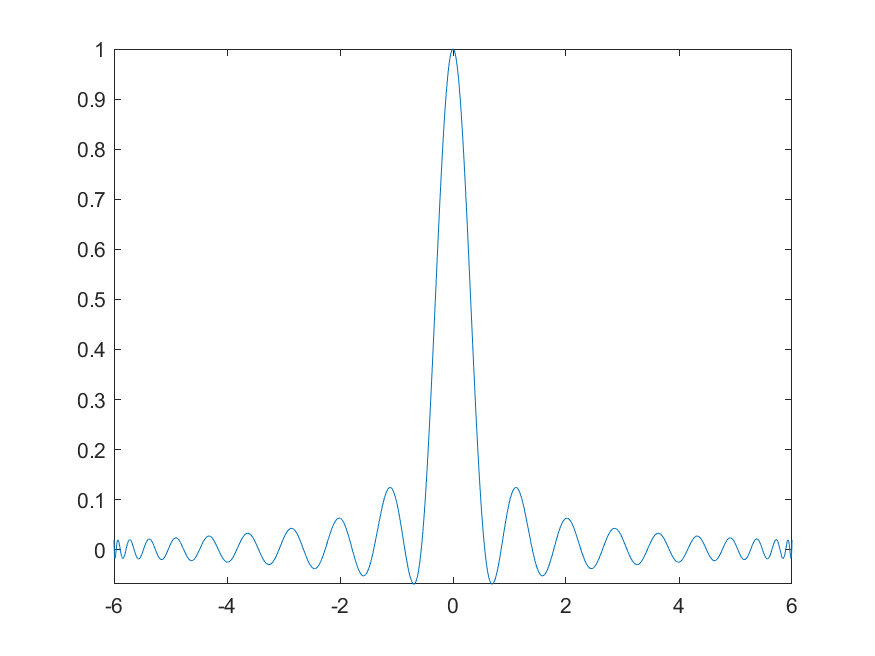
\includegraphics[scale=0.55]{cap4/4_7/40.png}
\end{center}
